\documentclass{beamer}
\graphicspath{{img/}}
\usepackage[latin1]{inputenc}
\usetheme{Marburg}
\title{Determining the long term cost of vaccination schedules}
\subtitle{A case study of measles in the United Kingdom}
\author{Max Goulding}
\date{Thursday 26th April, 2012}
\begin{document}

\begin{frame}
\titlepage
\end{frame}

\section{Introduction}
\begin{frame}{Measles}
\centering
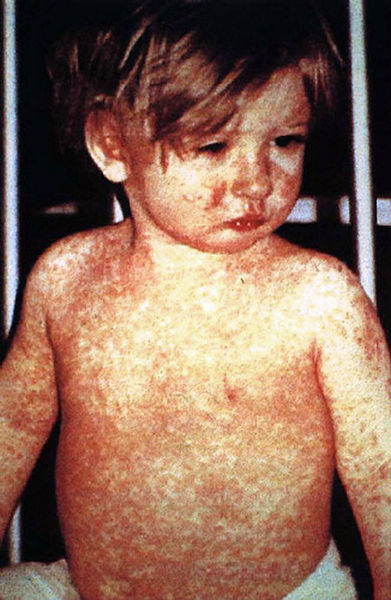
\includegraphics[width=45mm]{measleseuropean.jpg}
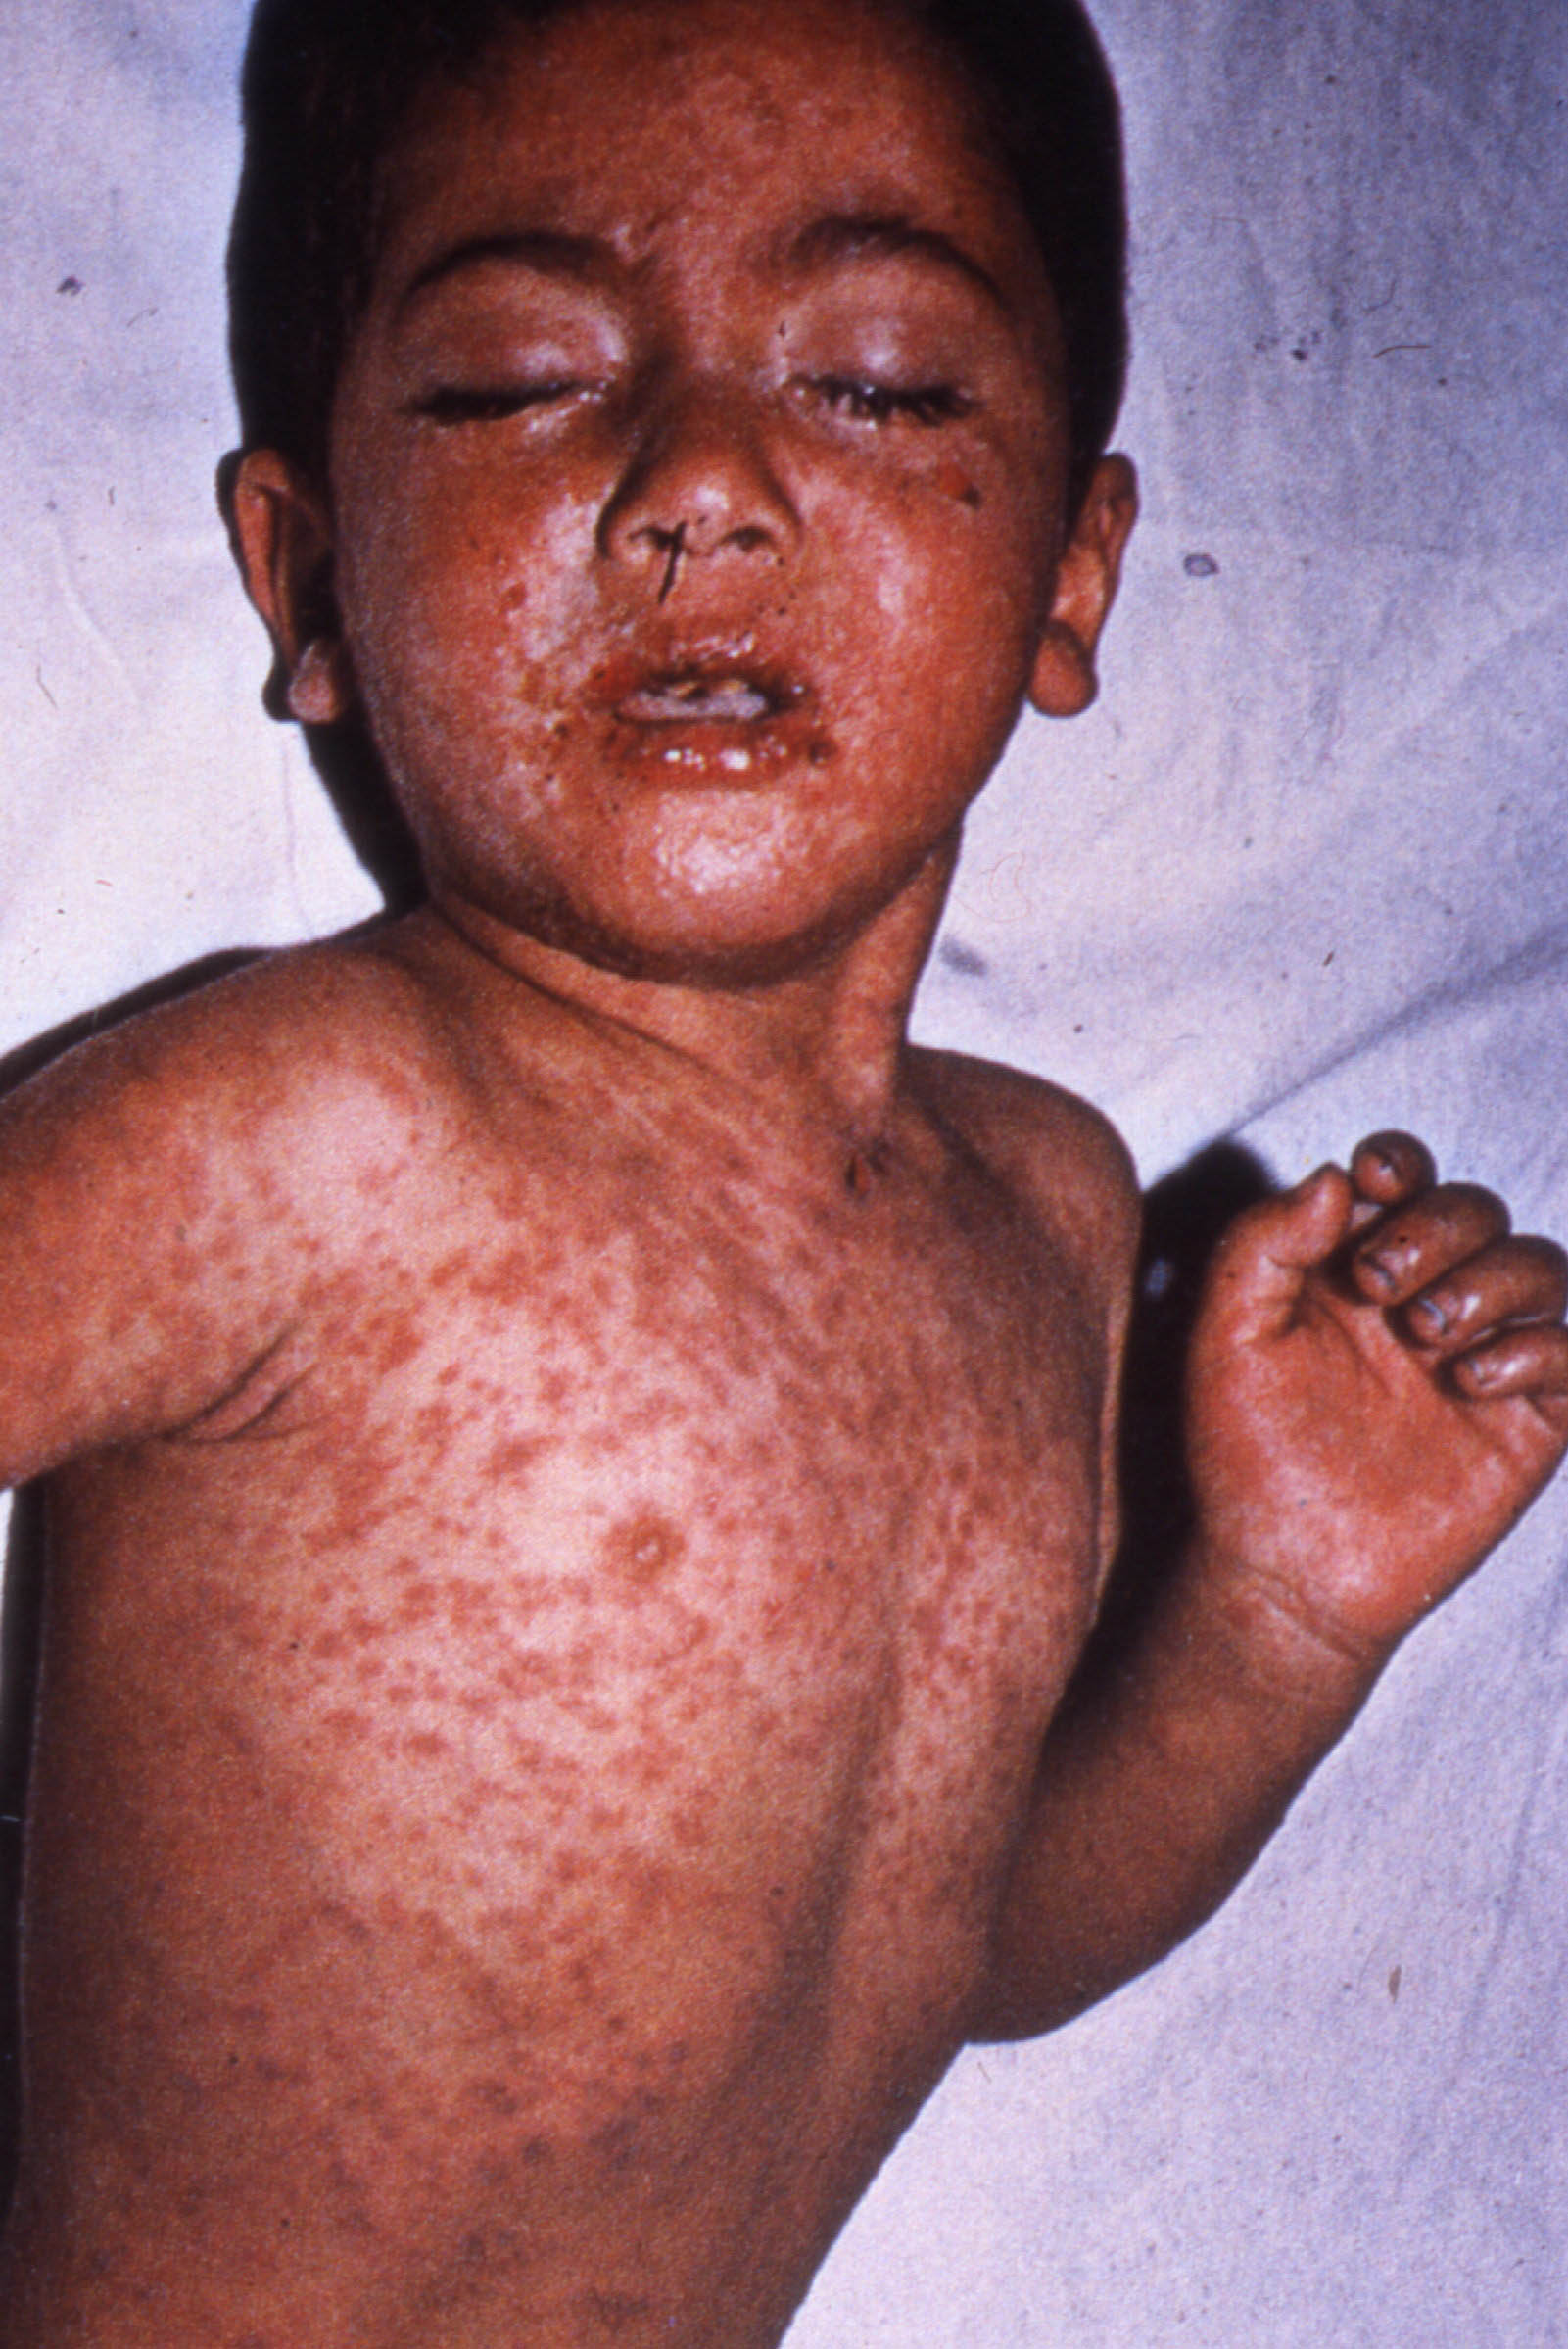
\includegraphics[width=46.1mm]{measleschild.jpg}
\end{frame}

\begin{frame}{Measles}
\begin{itemize}
\item{Highly infectious viral illness}
\item{Extremely unpleasant}
\item{Cold like symptoms / red eyes / light sensitivity / fever / spots in the mouth and throat}
\item {Complications such as pneumonia. In rare cases death}
\item{Complications when pregnant women are infected. Low birth weight. Premature birth. Miscarriage}
\end{itemize}
\end{frame}

\begin{frame} {Vaccination}
\begin{itemize}
\item {Before vaccination 200,000-700,000 notified infections and 30-300 deaths annually}
\item{Vaccine introduced in 1968. Replaced by MMR in 1988}
\item{Between 1998-2008, 2000-5000 notified cases and 0-3 deaths annually}
\item{89\% of infants vaccinated in 2010/2011}
\item{Current HPA recommendation first dose at 13 months and follow up 3-5 years}
\end{itemize}
\end{frame}

\begin{frame} {Maternal Antibodies}
\begin{itemize}
\item {Mother transfers antibodies to infant in the womb}
\item {Mothers with high antibody titre generally have infants with high antibody titre and vice versa}
\item {Maternal antibodies protect infants from infection and from successful vaccination}
\item {Maternal antibodies decay over time}
\item {Vaccination is often successful when an infant is no longer protected by maternal antibodies}
\item {Window of susceptibility}
\end{itemize}
\end{frame}

\begin{frame} {Impact of vaccination of maternal antibodies}
\begin{itemize}
\item{Since the introduction of vaccination there has been a decline in antibody titre within population}
\item {Vaccinated individuals have lower antibody titre than those who gain immunity through infection}
\item {Lack of natural boosting}
\item{Infants have lower maternal antibody levels}
\item {Infants lose immunity sooner than prior vaccination}
\item {Increased window of susceptibility}
\end{itemize}
\end{frame}

\section{Project breakdown}
\begin{frame} {Project task}
\begin{quote}
Should vaccination schedules be altered to account for the increased window of susceptibility in infants?
\end{quote}

\begin{itemize}
\pause \item{\alert{Model} different vaccination schedules for measles}
\item{Determine which offers \alert{optimum} results}
\end{itemize}
\end{frame}

\begin{frame} {Optimum?}
What different ways are there to determine optimum results?
\begin{itemize}
 \item{Minimise number of infections}
 \item{Minimise number of infections to particular age groups, as certain groups may have greater risks if infected}
 \item{Speed to eradication}
 \item{Minimise overall cost of measles}
\end{itemize}
\end{frame}

\begin{frame} {How to model}
There are two main possibilities to model diseases where the initial conditions are known.
\begin{itemize}
\item{Stochastic}
\item{\alert{Differential}}
\end{itemize}
\end{frame}

\section{Model development}
\begin{frame} {General Methods}
I use some common methods throughout :
\begin{itemize}
\item{Model using ODEs}
\item{All ODEs are solved using a fourth order Runge-Kutta method, with time step $h=\frac{1}{365}$}
\item{Stable population of 60,000,000}
\item{Initial values of $S=6,400,000$, $I=600,000$ and $R=53,000,000$}
\end{itemize}
\end{frame}
\subsection{SIR}
\begin{frame} {SIR} {Assumptions}
\begin{itemize}
	\item{The population is divided up into three group :
	\begin{itemize}
	 \item{Susceptible}
	 \item{Infectious}
	 \item{Recovered}
	\end{itemize}}
	\item{Transitions from groups are exponential decays}
	\item{Homogeneous mixing}	
	\item{Individuals born susceptible}
	\item{Recovered immunity lifelong}
	\item{Death applies equally to each group}	
\end{itemize}
\end{frame}

\begin{frame} {SIR} {Model}
\begin{figure}
\centering
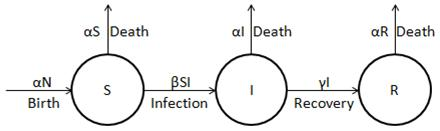
\includegraphics[width=70mm]{simpleSIRModel.jpg}
\label{fig:simpleSIRpictoral}
\end{figure}
\begin{align*} 
N &= S + I + R \\
\frac{dS}{dt} &= \alpha N - \beta SI - \alpha S \\ 
\frac{dI}{dt} &= \beta SI - \gamma I - \alpha I \\ 
\frac{dR}{dt} &= \gamma I - \alpha R
\end{align*}
\end{frame}

\begin{frame} {SIR} {Results}
\begin{figure}
\centering
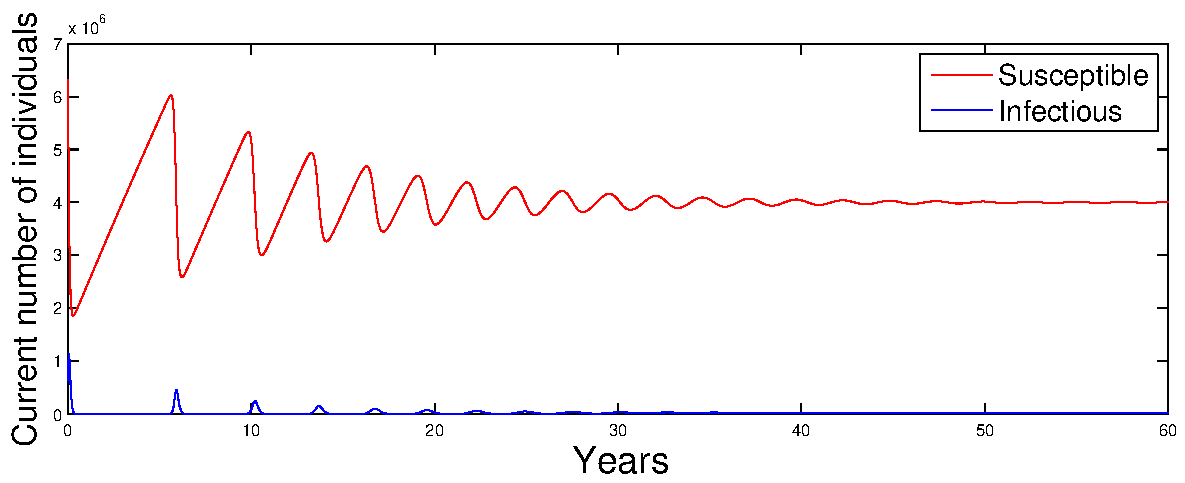
\includegraphics[width=100mm]{figsimpleSIR60}
\caption{The current number of infectious and susceptible individuals at each time step. Initial values of $S=6,400,000$, $I=600,000$ and $R=53,000,000$.}
\end{figure}
\end{frame}

\begin{frame} {SIR} {Challenges}
Does NOT account for vaccination!!!
\end{frame}

\subsection{SVIR}
\begin{frame} {SVIR} {Assumptions}
\begin{itemize}
\item {Inclusion of a Vaccinated group, $V$}
 \item{Vaccination occurs at birth}
 \item {Vaccination is always successful}
 \item {$p$ proportion of the population are vaccinated}
 \item {Vaccinated immunity is lifelong}
\end{itemize}
\end{frame}

\begin{frame} {SVIR} {Model}
\begin{figure}
\centering
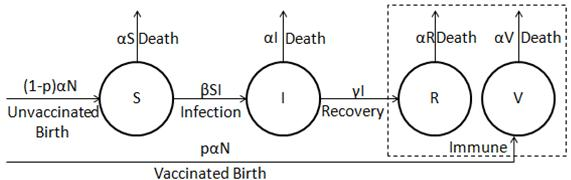
\includegraphics[width=90mm]{SVIRModel.jpg}
\label{fig:SVIRpictoral}
\end{figure}
\begin{align*}
N &= S + V + I + R \\
\frac{dS}{dt} &= (1-p)\alpha N - \beta SI - \alpha S \\ 
\frac{dV}{dt} &= p\alpha N - \alpha V \\ 
\frac{dI}{dt} &= \beta SI - \gamma I - \alpha I \\ 
\frac{dR}{dt} &= \gamma I - \alpha R 
\end{align*}
\end{frame}

\begin{frame} {SVIR} {Results}
\begin{figure}
\centering
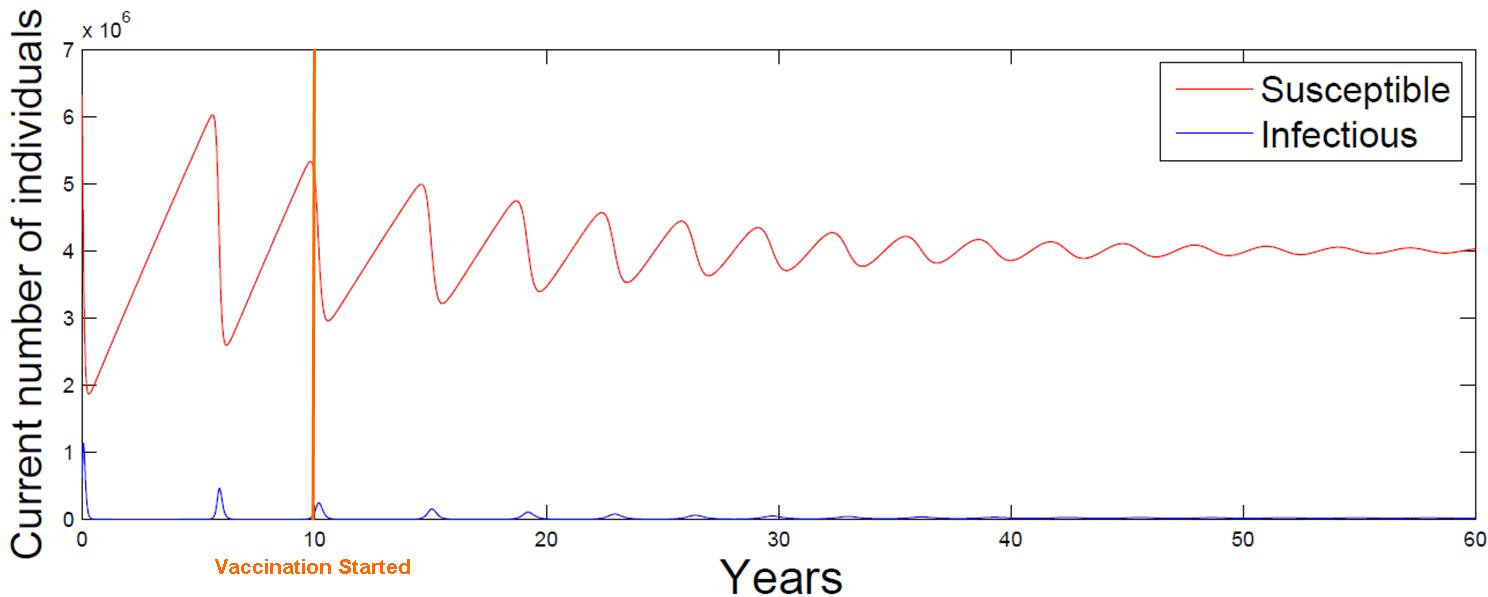
\includegraphics[width=100mm]{figsvir30.jpg}
\caption{The current number of infectious and susceptible individuals at each time step. 30\% vaccination introduced in 10th year. Initial values of $S=6,400,000$, $V=0$, $I=600,000$ and $R=53,000,000$.}
\end{figure}
\end{frame}

\begin{frame} {SVIR} {Results}
\begin{figure}
\centering
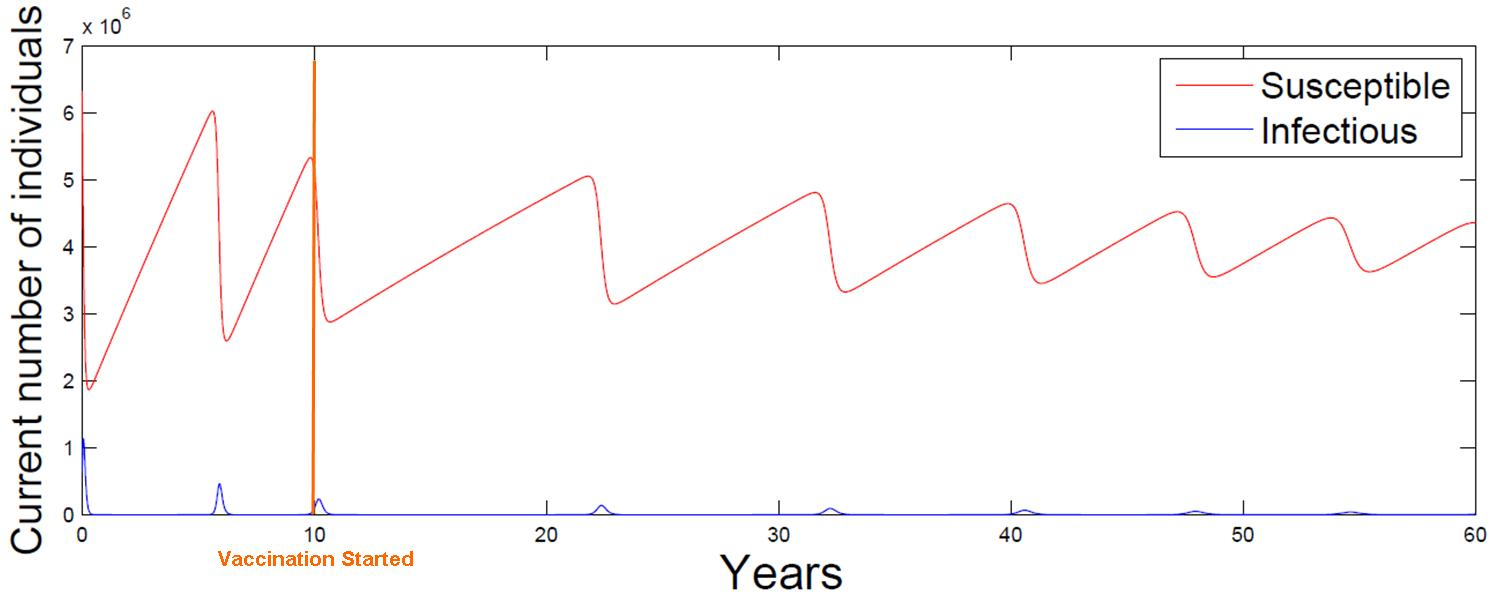
\includegraphics[width=100mm]{figsvir70.jpg}
\caption{The current number of infectious and susceptible individuals at each time step. 70\% vaccination introduced in 10th year. Initial values of $S=6,400,000$, $V=0$, $I=600,000$ and $R=53,000,000$.}
\end{figure}
\end{frame}

\begin{frame} {SVIR} {Results}
\begin{figure}
\centering
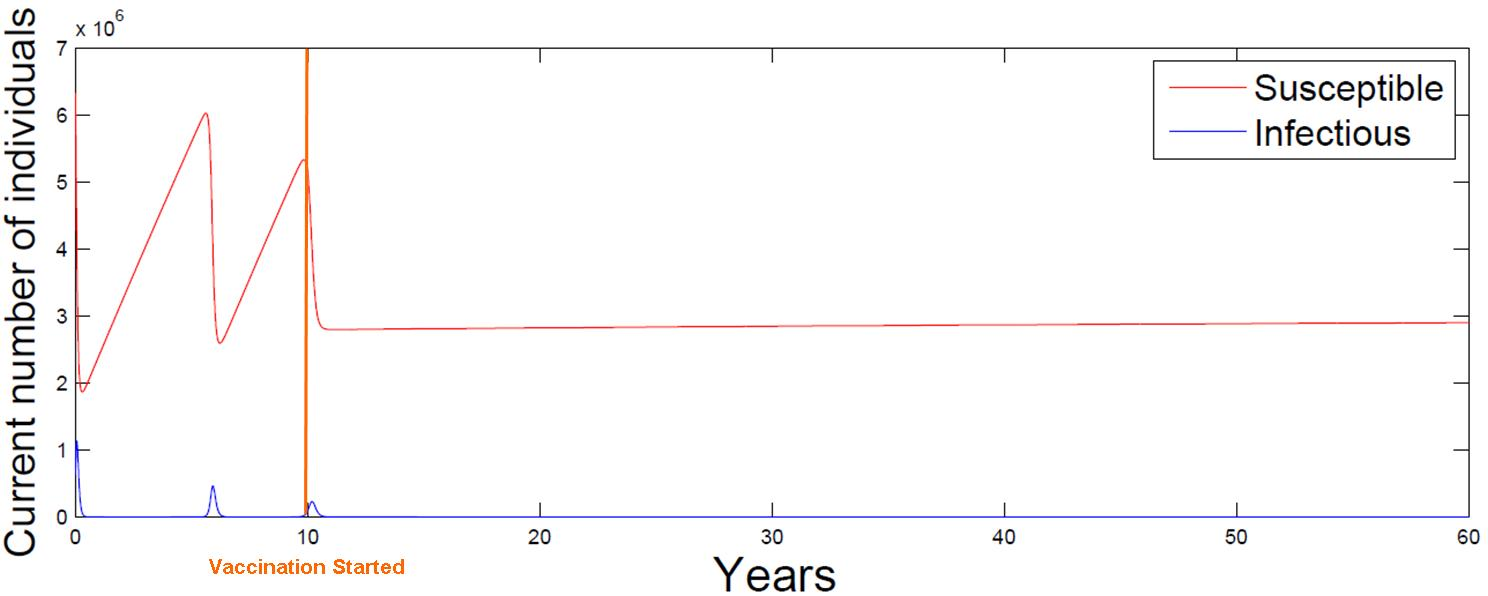
\includegraphics[width=100mm]{figsvir95.jpg}
\caption{The current number of infectious and susceptible individuals at each time step. 95\% vaccination introduced in 10th year. Initial values of $S=6,400,000$, $V=0$, $I=600,000$ and $R=53,000,000$.}
\end{figure}
\end{frame}

\begin{frame} {SVIR} {Overall cost results}
\begin{figure}
\centering
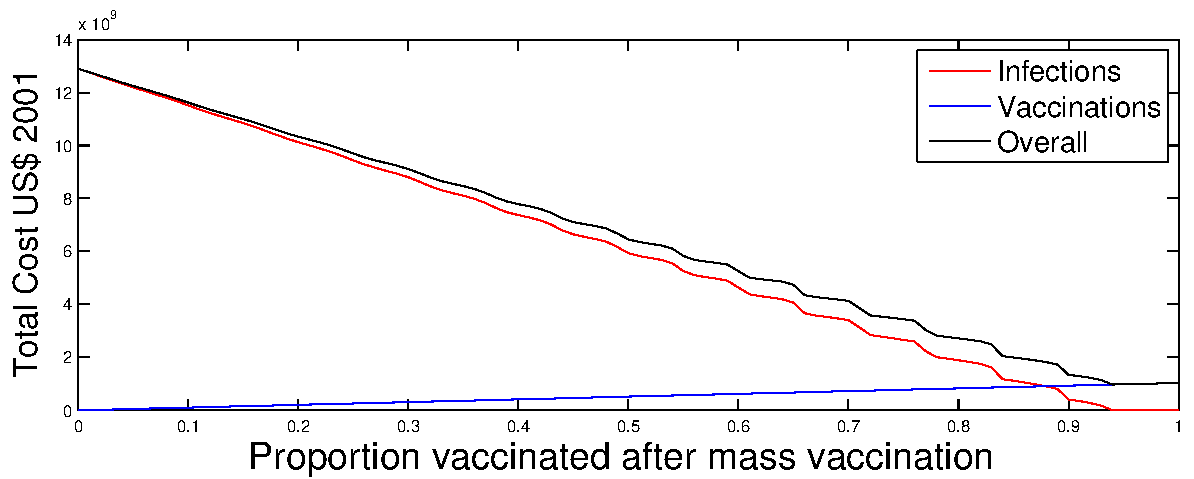
\includegraphics[width=100mm]{figproportionSVIRcost0to100}
\caption{Total cost of varying proportions of vaccination. The system is run for 50 years after mass vaccination. US \$307 (2001 levels) per measles case, US \$22.1 (2001 levels) per vaccination and US \$2.08 (2001 levels) per associated cost of vaccination.}
\end{figure}
\end{frame}

\begin{frame} {SVIR} {Overall cost results}
\begin{figure}
\centering
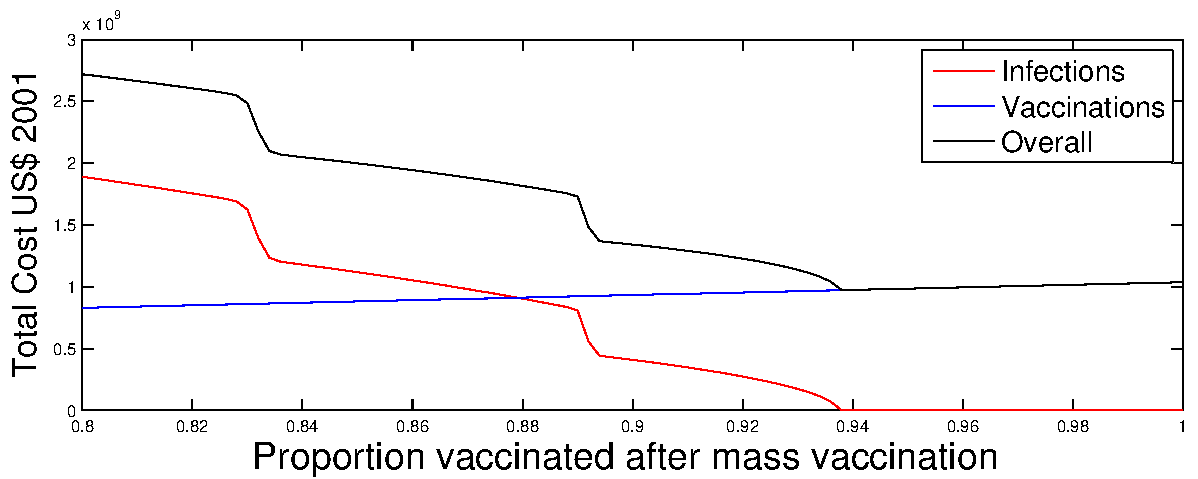
\includegraphics[width=100mm]{figproportionSVIRcost80to100}
\caption{Total cost of varying proportions of vaccination. The system is run for 50 years after mass vaccination. US \$307 (2001 levels) per measles case, US \$22.1 (2001 levels) per vaccination and US \$2.08 (2001 levels) per associated cost of vaccination.}
\end{figure}
\end{frame}

\begin{frame} {SVIR} {Challenges}
Does NOT take account of protective maternal immunity!!!
\end{frame}

\subsection{Ideal BSVIR}
\begin{frame} {Ideal BSVIR} {Assumptions}
\begin{itemize}
\item {Inclusion of birth immunity groups, $B_R$ and $B_V$ for infants of recovered and vaccinated mothers respectively}
 \item{Only individuals from $S$, $R$ and $V$ groups give birth with infants entering $S$, $B_R$ and $B_V$ groups respectively}
 \item{Births weighted to maintain stable population}
 \item{Birth recovered and vaccinated immunity exponentially decays at rate $\sigma$ and $\xi$ respectively}
 \item{Vaccination occurs when individuals become susceptible}
\end{itemize}
\end{frame}

\begin{frame} {Ideal BSVIR} {Model}
\begin{figure}
\centering
\includegraphics[width=100mm]{IdealBSVIRmodel.jpg}
\end{figure}
\end{frame}

\begin{frame} {Ideal BSVIR} {Model}
\begin{align*}
N &= B_R + B_V + S + V + I + R \\
\frac{dB_R}{dt} &= \frac{\alpha N R}{\left( S+V+R \right)} - \sigma B_R - \alpha B_R\\
\frac{dB_V}{dt} &= \frac{\alpha N V}{\left( S+V+R \right)} - \xi B_V - \alpha B_V\\
\frac{dS}{dt} &= (1-p) \left(\frac{\alpha N S}{\left( S+V+R \right)} + \sigma B_R + \xi B_V\right)- \beta SI - \alpha S \\ 
\frac{dV}{dt} &= p \left(\frac{\alpha N S}{\left( S+V+R \right)} + \sigma B_R + \xi B_V\right) - \alpha V \\ 
\frac{dI}{dt} &= \beta SI - \gamma I - \alpha I \\ 
\frac{dR}{dt} &= \gamma I - \alpha R 
\end{align*}
\end{frame}

\begin{frame} {Ideal BSVIR} {Results}
\begin{figure}
\centering
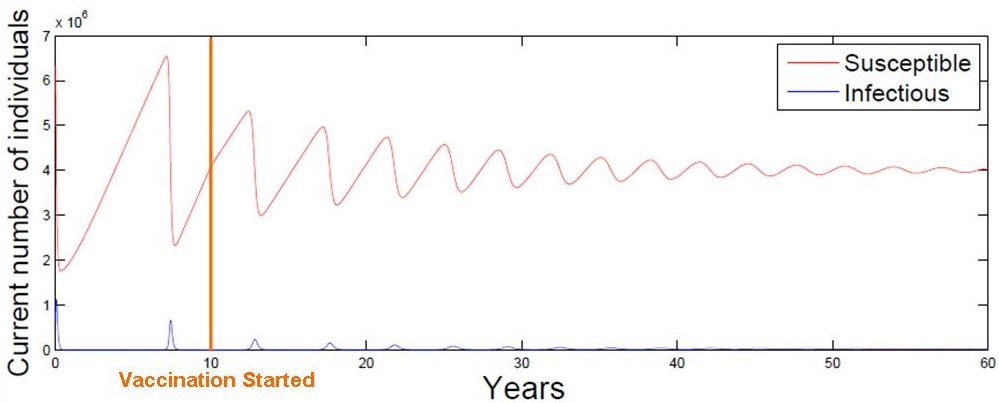
\includegraphics[width=100mm]{figidealbsvir30.jpg}
\caption{The current number of infectious and susceptible individuals at each time step. 30\% vaccination introduced in 10th year. Initial values of $B_R=0$, $B_V=0$, $S=6,400,000$, $V=0$, $I=600,000$ and $R=53,000,000$.}
\end{figure}
\end{frame}

\begin{frame} {Ideal BSVIR} {Results}
\begin{figure}
\centering
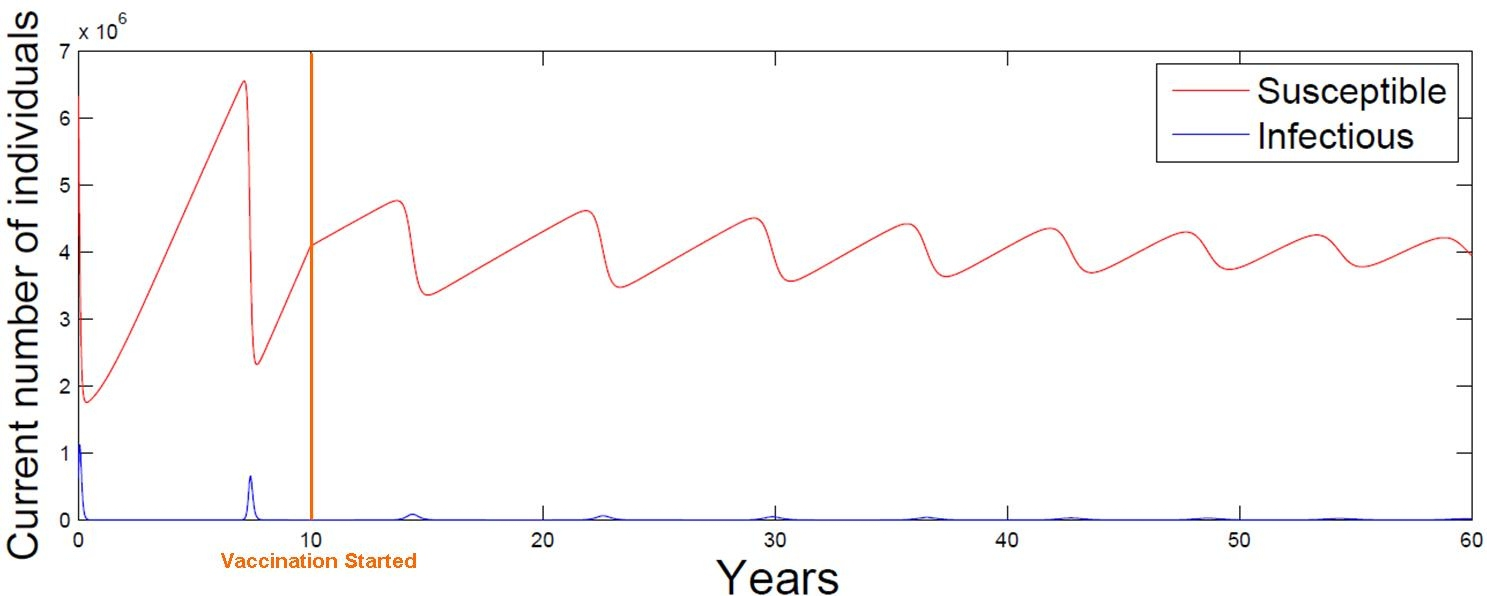
\includegraphics[width=100mm]{figidealbsvir70.jpg}
\caption{The current number of infectious and susceptible individuals at each time step. 70\% vaccination introduced in 10th year. Initial values of  $B_R=0$, $B_V=0$, $S=6,400,000$, $V=0$, $I=600,000$ and $R=53,000,000$.}
\end{figure}
\end{frame}

\begin{frame} {Ideal BSVIR} {Results}
\begin{figure}
\centering
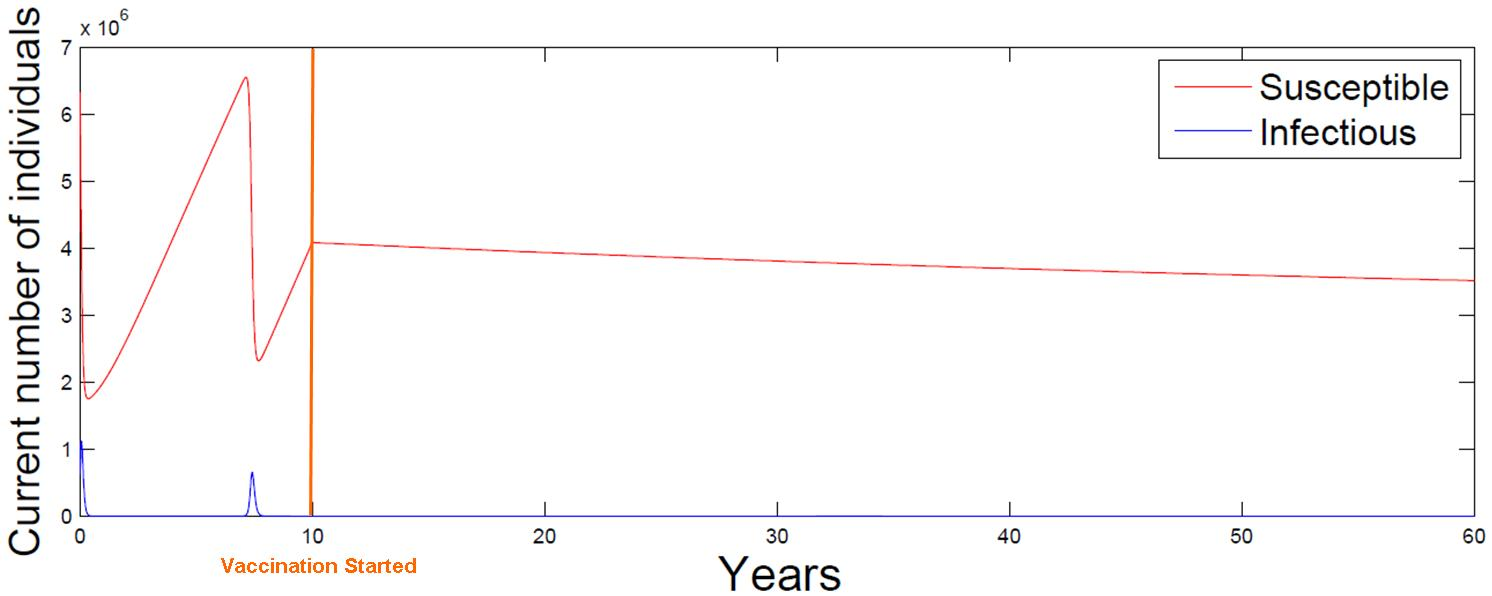
\includegraphics[width=100mm]{figidealbsvir95.jpg}
\caption{The current number of infectious and susceptible individuals at each time step. 95\% vaccination introduced in 10th year. Initial values of  $B_R=0$, $B_V=0$, $S=6,400,000$, $V=0$, $I=600,000$ and $R=53,000,000$.}
\end{figure}
\end{frame}

\begin{frame} {Ideal BSVIR} {Overall cost results}
\begin{figure}
\centering
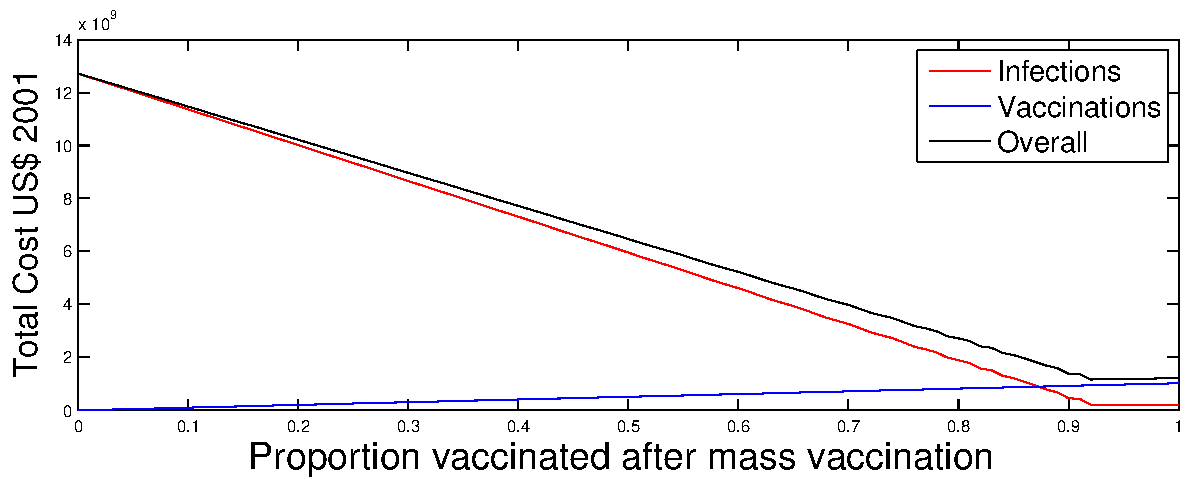
\includegraphics[width=100mm]{figproportionidealBSVIRcost0to100}
\caption{Total cost of varying proportions of vaccination. The system is run for 50 years after mass vaccination. US \$307 (2001 levels) per measles case, US \$22.1 (2001 levels) per vaccination and US \$2.08 (2001 levels) per associated cost of vaccination.}
\end{figure}
\end{frame}

\begin{frame} {Ideal BSVIR} {Overall cost results}
\begin{figure}
\centering
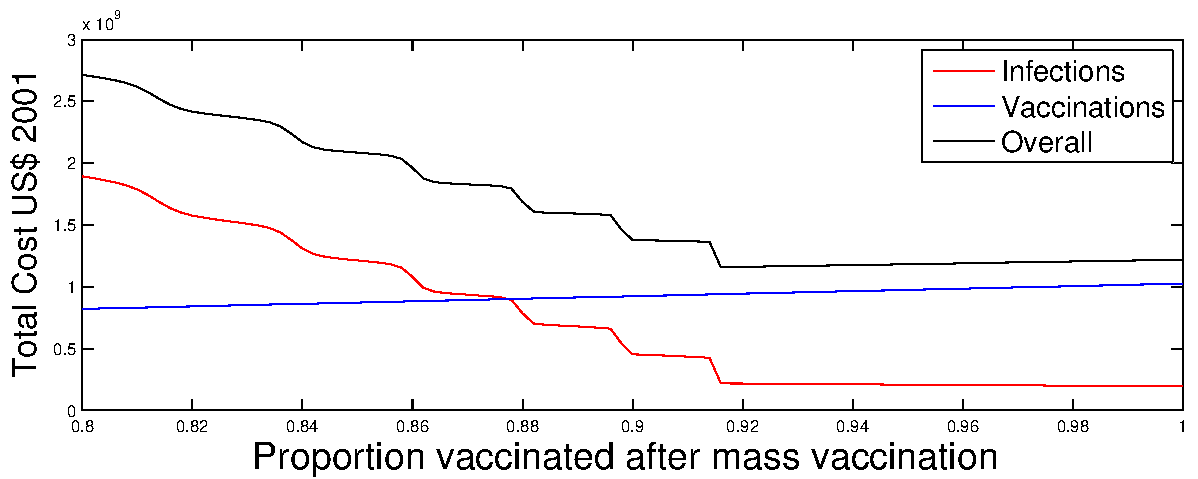
\includegraphics[width=100mm]{figproportionidealBSVIRcost80to100}
\caption{Total cost of varying proportions of vaccination. The system is run for 50 years after mass vaccination. US \$307 (2001 levels) per measles case, US \$22.1 (2001 levels) per vaccination and US \$2.08 (2001 levels) per associated cost of vaccination.}
\end{figure}
\end{frame}

\begin{frame} {Ideal BSVIR} {Challenges}
Vaccination schedules are NOT realistic.

Loss of maternal immunity NOT realistic.
\end{frame}

\subsection{Realistic BSVIR}
\begin{frame} {Realistic BSVIR} {Assumptions}
\begin{itemize}
\item {Have an age-stratified model}
\item{Store population as a matrix, with rows as immunity statuses and columns as age groups}
\item{Age groups the same size as the time step}
\item{Discretely apply vaccination to the appropriate age group(s). Only those susceptible have successful vaccination}
\item{Only those in certain age groups give birth}
\item{For double vaccination schedules, assume second vaccination is independent}                        
\item{For computational reasons use a `partially' age-stratified model, with those $>$ 4 years in s single group}
\end{itemize}
\end{frame}

\begin{frame} {Realistic BSVIR} {Model}
\begin{figure}
\centering
\includegraphics[width=95mm]{realisticBSVIRmodel.jpg}
\end{figure}
\end{frame}

\begin{frame} {Realistic BSVIR} {Results}
\begin{figure}
\centering
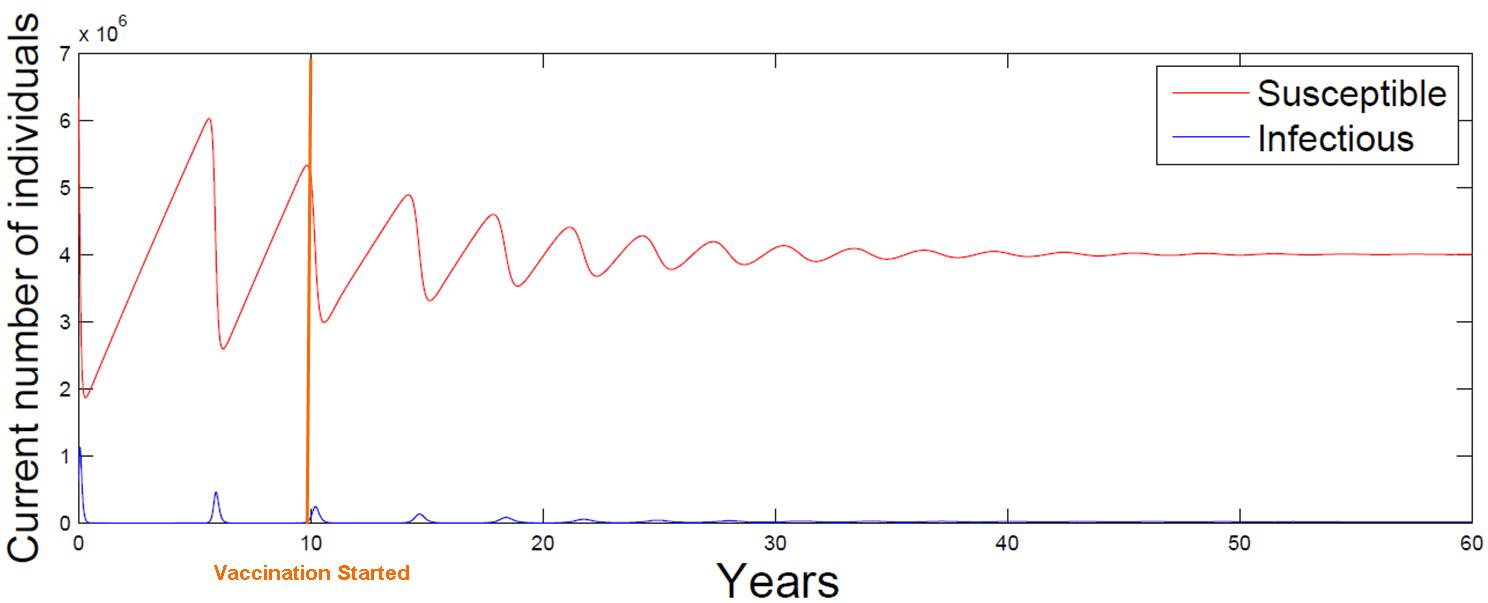
\includegraphics[width=100mm]{figrealisticbsvir30.jpg}
\caption{The current number of infectious and susceptible individuals at each time step. 30\% vaccination introduced in 10th year. Initial values of $S\left( n \right) =6,400,000$, $I\left( n \right) =600,000$, $R\left( n \right) =53,000,000$ and $B_V\left( n \right) =B_R\left( n \right) =V\left( n \right) =0$, where n is $>4$ age group.}
\end{figure}
\end{frame}

\begin{frame} {Realistic BSVIR} {Results}
\begin{figure}
\centering
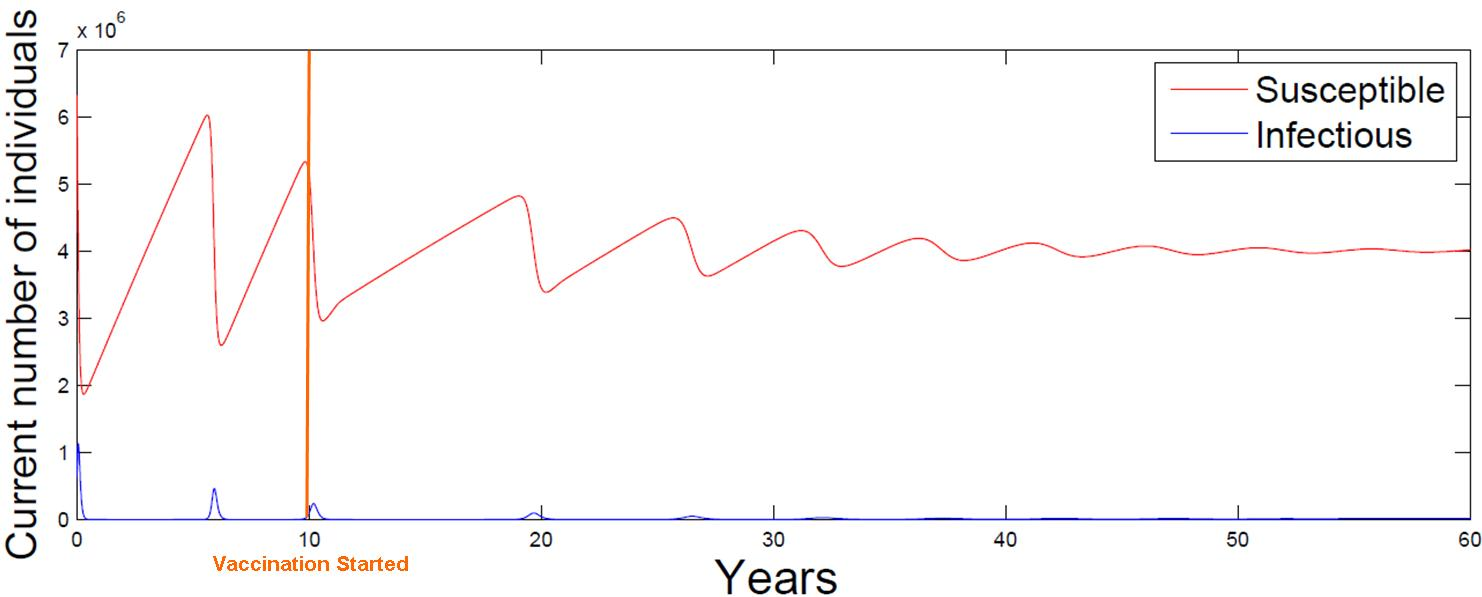
\includegraphics[width=100mm]{figrealisticbsvir70.jpg}
\caption{The current number of infectious and susceptible individuals at each time step. 70\% vaccination introduced in 10th year. Initial values of $S\left( n \right) =6,400,000$, $I\left( n \right) =600,000$, $R\left( n \right) =53,000,000$ and $B_V\left( n \right) =B_R\left( n \right) =V\left( n \right) =0$, where n is $>4$ age group.}
\end{figure}
\end{frame}

\begin{frame} {Realistic BSVIR} {Results}
\begin{figure}
\centering
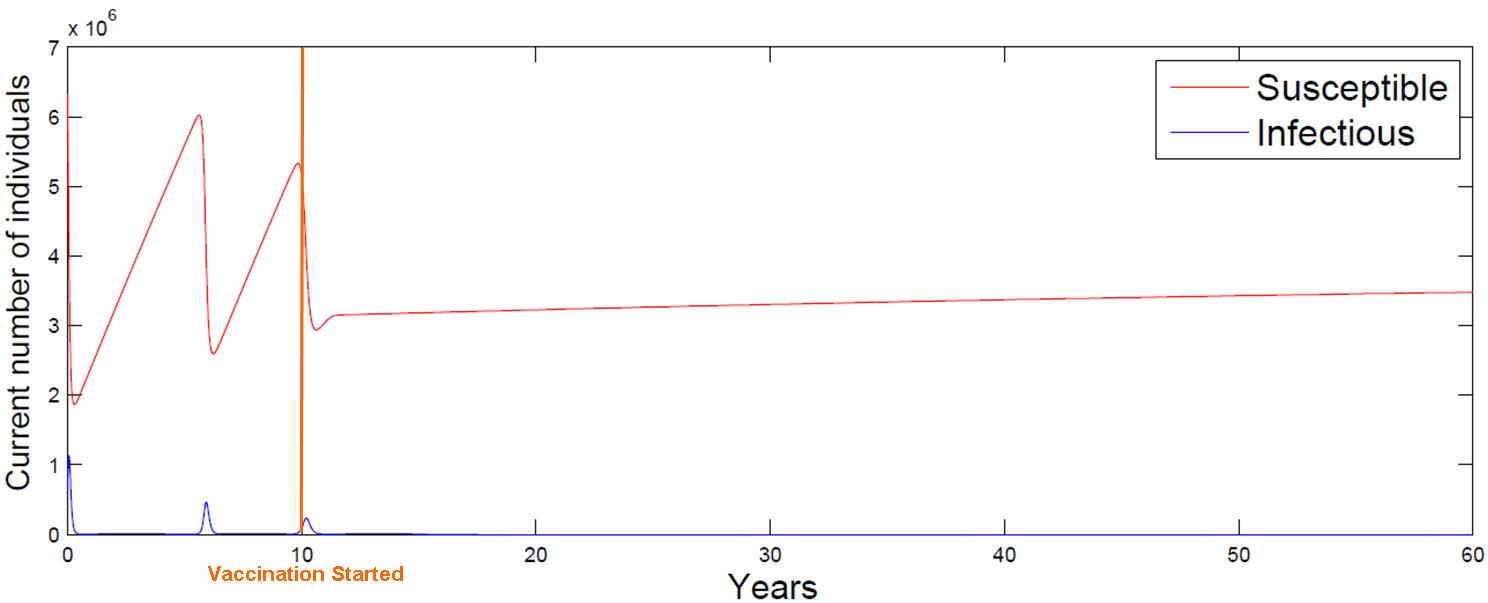
\includegraphics[width=100mm]{figrealisticbsvir95.jpg}
\caption{The current number of infectious and susceptible individuals at each time step. 95\% vaccination introduced in 10th year. Initial values of $S\left( n \right) =6,400,000$, $I\left( n \right) =600,000$, $R\left( n \right) =53,000,000$ and $B_V\left( n \right) =B_R\left( n \right) =V\left( n \right) =0$, where n is $>4$ age group.}
\end{figure}
\end{frame}

\begin{frame} {Realistic BSVIR} {Overall cost results}
\begin{figure}
\centering
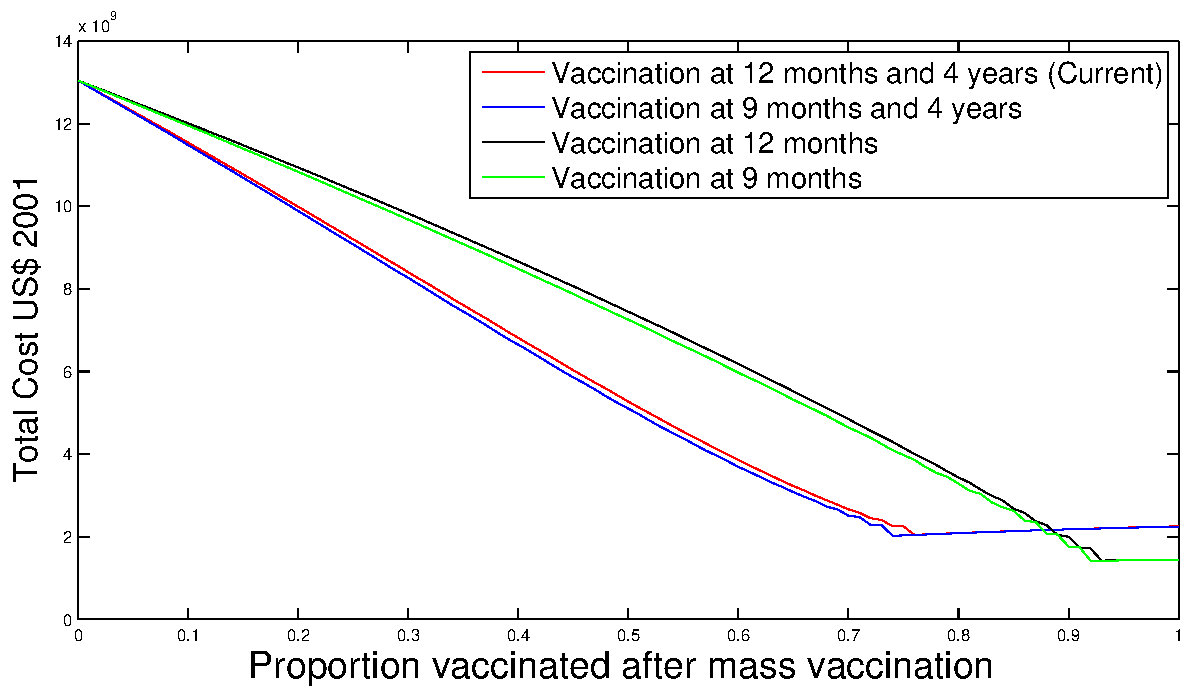
\includegraphics[width=90mm]{figproportionrealisticBSVIRcomparison0to100}
\caption{Total cost of varying proportions of vaccination. The system is run for 50 years after mass vaccination. US \$307 (2001 levels) per measles case, US \$22.1 (2001 levels) per vaccination and US \$2.08 (2001 levels) per associated cost of vaccination.}
\end{figure}
\end{frame}

\begin{frame} {Realistic BSVIR} {Overall cost results}
\begin{figure}
\centering
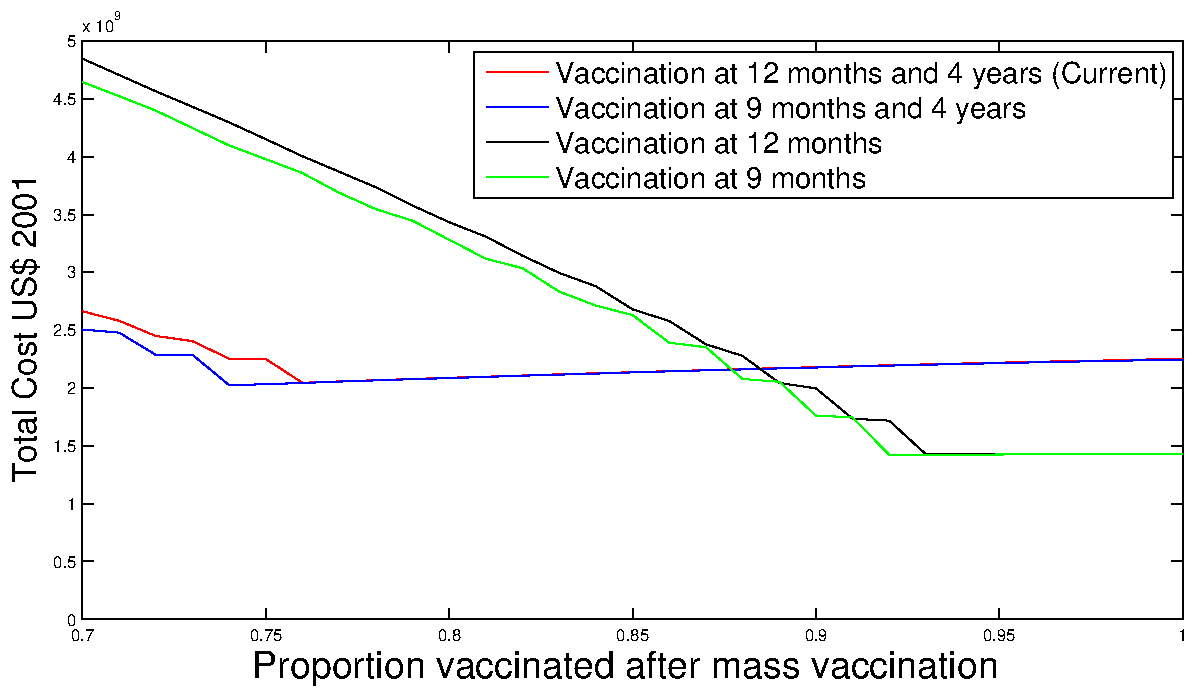
\includegraphics[width=90mm]{figproportionrealisticBSVIRcomparison70to100}
\caption{Total cost of varying proportions of vaccination. The system is run for 50 years after mass vaccination. US \$307 (2001 levels) per measles case, US \$22.1 (2001 levels) per vaccination and US \$2.08 (2001 levels) per associated cost of vaccination.}
\end{figure}
\end{frame}

\begin{frame} {Realistic BSVIR} {Challenges}
\begin{itemize}
\item{Not fully age-stratified}
 \item{Serological data not up to date}
 \item{Double vaccination schemes independent}
 \item{Population assumptions over simplistic}
 \item{Economic factors not accounted for}
 \item{Lifelong immunity not guaranteed}
\end{itemize}
\end{frame}

\section{Conclusions}
\begin{frame}{Overall Results}
These models show some general trends :
\begin{itemize}
\item {It is cheaper in terms of overall cost to over-vaccinated a population than to under-vaccinated a population}
\item {Eradication is possible if over 95\% is vaccinated}
\item {Reduction of the initial vaccination to 9 months may have potential cost savings}
\item {Changing to a single vaccination schedule may bring a cost reduction if a high enough proportion of infants are vaccinated}
\end{itemize}
\end{frame}

\begin{frame}{Future Developments}
\begin{itemize}
	\item{Age-Stratified Models}
	\item{Up to date serological data}
	\item{Model mumps and rubella}
\end{itemize}
\end{frame}

\end{document}
